\newpage
\section{Problem 2: TEXTURE ANALYSIS}\label{problem-2-texture-analysis}
In this problem, there is an image \textbf{sample2.png} composed of several different textures.

Given an image, \nameref{sample2}.

Original image \nameref{sample2} for question \nameref{problem-2-texture-analysis}.
\begin{figure}
    \centering
    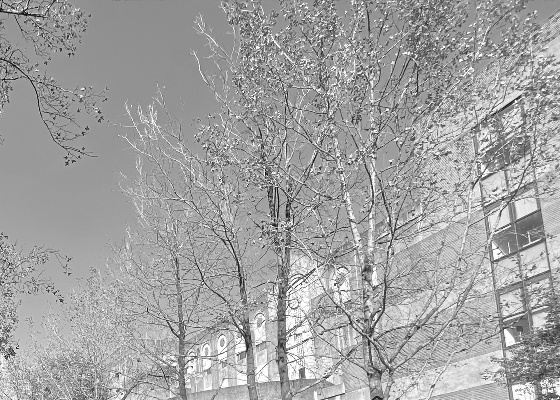
\includegraphics[width=0.7\textwidth]{src/sample2.png}
    \caption{\textbf{sample2.jpg}}
    \label{sample2}
\end{figure}

\subsection{(a)}\label{2_a}
Perform Law’s method on sample2.png to obtain the feature vector of each pixel and discuss the feature vectors in your report.

\paragraph{Motivation}
Micro-structure (Multi-channel) method. It emphasize the microstructure of the texture with \(9\)-types of \textbf{filtering} (low-pass/local average, edge detector/\(1^{\mbox{st}}\)-order, spot detector/\(2^{\mbox{st}}\)-order) then compute \textbf{energy distribution} of these subbands.

\paragraph{Approach}
We could follow the two steps of Law's method in \textit{Lec 5 page 16--25}.

\begin{enumerate}
    \item Convolution \(M_{i}(j, k) = F(j, k) \otimes H_{i}(j, k) \). \\
	where \(H_{i}(j, k)\) is \textbf{micro-structure impulse} response arrays.
    \item Energy computation with \(T_{i}(j, k) = \sum_{(m, n) \in w} |M_{i}(j+m, k+n) |^{2} \). \\
	where \(w\) is \textbf{window size}.
\end{enumerate}

\paragraph{Performance of results}
In the end, I choose the window size \(w = 13\).

Result of problem 2(a):

\textbf{Shape}: \((400, 600, 9)\)
We could see the Law's method generate \(9\) features for each pixel.

\textbf{Statistics}:
\begin{table}[]
%\begin{tabular}{l|l|l|l|l|l|l|l|l|l|}
\begin{adjustwidth}{-2cm}{}
\begin{tabularx}{\paperwidth}{X|l|l|l|l|l|l|l|l|l|}
\cline{2-10}
                           & feature 1  & feature 2 & feature 3 & feature 4 & feature 5 & feature 6 & feature 7 & feature 8 & feature 9 \\ \hline
\multicolumn{1}{|l|}{mean} & 632578.51  & 12606.37  & 10740.66  & 12496.21  & 14566.39  & 17710.59  & 10324.98  & 18076.89  & 30689.82  \\ \hline
\multicolumn{1}{|l|}{std}  & 255219.15  & 14841.65  & 12589.02  & 14507.87  & 16546.63  & 19929.37  & 11479.35  & 19661.54  & 33759.59  \\ \hline
\multicolumn{1}{|l|}{min}  & 24443.18   & 5.72      & 10.08     & 5.4       & 14.94     & 28.06     & 10.03     & 24.63     & 46.38     \\ \hline
\multicolumn{1}{|l|}{25\%} & 503566.26  & 111.81    & 114.33    & 222.96    & 189.88    & 227.88    & 178.12    & 264.81    & 391.8     \\ \hline
\multicolumn{1}{|l|}{50\%} & 741495.28  & 3197.15   & 3338.21   & 3865.16   & 4423.5    & 6215.19   & 4084.01   & 7322.06   & 12601.59  \\ \hline
\multicolumn{1}{|l|}{75\%} & 818331.18  & 26522.01  & 21761.25  & 25030.34  & 30454.5   & 36466.03  & 20445.08  & 36738.09  & 61693.36  \\ \hline
\multicolumn{1}{|l|}{max}  & 1168527.54 & 65892.08  & 73024.13  & 122812.59 & 72651.31  & 89798     & 69072.48  & 91929.81  & 145748.75 \\ \hline
%\end{tabular}
\end{tabularx}
\caption{Prob 2(a) Summary statistics}
\label{table:prob2a}
\end{adjustwidth}
\end{table}
I export summary statistics to the \texttt{tmp/prob2a\_stats.csv}.

The \nameref{table:prob2a} tell us:
\begin{itemize}
    \item We could see the \textbf{feature 1/ LP\(\times\)LP} is relative larger than other features. With mean \(632578\).
    \item The \textbf{feature 9/ HP\(\times\)HP} is second large features. And its \textbf{standard deviation} is largest one and only one that larger than its mean. With std \(33759\).
\end{itemize}

Then we could observe the \textbf{scatters} \nameref{prob2a_scatter_matrix} to get the correlation between features.
\begin{figure}
    \centering
    \includegraphics[width=0.5\textwidth]{src/tmp/prob2a_scatter_matrix.png}
    \caption{Scatter matrix}
    \label{prob2a_scatter_matrix}
\end{figure}

\begin{itemize}
    \item Most of features are \textbf{positive skew}. Only \textbf{feature 1} is relative uniform.
    \item It seems \textbf{feature 9} are positive correlative with \textbf{feature 4, 5, 7}.
\end{itemize}

Then, we observe the \textbf{outlier} \nameref{prob2a_boxplot} of each features.
\begin{figure}
    \centering
    \includegraphics[width=0.5\textwidth]{src/tmp/prob2a_boxplot.png}
    \caption{Box plot}
    \label{prob2a_boxplot}
\end{figure}
We could see the \textbf{feature 3/ LP\(\times\)HP} have \(2\) \textbf{larger outliers} than others.

Finally, we observe the \textbf{probability–probability plot} \nameref{prob2a_probplot} to evaluate the skewness of a distribution.
\begin{figure}
    \centering
    \includegraphics[width=0.5\textwidth]{src/tmp/prob2a_probplot.png}
    \caption{Probability plot}
    \label{prob2a_probplot}
\end{figure}
We could check if we \textbf{remove/drop} \(0\) values, most of our features are not skew. The special features are 
\begin{itemize}
    \item \textbf{feature 1} which is original uniform than others.
    \item \textbf{feature 4/ BP\(\times\)LP} is skew up.
\end{itemize}
For this result, we could design \textbf{row features} to enhance our performance when classifying.

\paragraph{Discussion}
I'm not sure the scale/normalization of \(F_{j, k} \in [0, 255]\) or \(F_{j, k} \in [0, 1]\). My intuition tells me the difference occurs at \textbf{energy computation}.
Unfortunately, I keep this issue in future.


\subsection{(b)}\label{2_b}
Use k-means algorithm to classify each pixel with the feature vectors you obtained from (a). Label same kind of texture with the same color and output it as \textbf{result3.png}.

\paragraph{Motivation}
Un-supervised texture classification. The good classification is \textbf{large inter-clustering} as well as \textbf{small intra-clustering}. Follow the characteristics of this image, we could choose \(k=4\) or \(k=4\) as our parameter.


\paragraph{Approach}
Follow \href{https://gist.github.com/tvwerkhoven/4fdc9baad760240741a09292901d3abd}{this gist},
\begin{enumerate}
    \item Initialize \(k\) vectors as the initial centroids. This approach select the \textbf{existing points} in training data.
    \item With \texttt{maxIters} iterative times:
	\begin{itemize}
	    \item Form \(k\) clusters using nearest neighbor rule.
	    \item re-compute the centroid of each cluster.
	\end{itemize}
\end{enumerate}
After we get the result of clusters, I use \texttt{matplotlib.plt.cmap} to assign the colors for each cluster.

\paragraph{Performance of results}
In the end, I choose the \(k=4\).

Result of problem 2(b): \nameref{result3}.
\begin{figure}
    \centering
    \includegraphics[width=0.7\textwidth]{src/result3_report.png}
    \caption{\textbf{result3.png} K-means of Law's method}
    \label{result3}
\end{figure}
The top \textit{sky} is similar to \textit{flowers}. It seem not a good approach.

\paragraph{Discussion}
For \(k=5\), we have \nameref{result3_keq5}
\begin{figure}
    \centering
    \includegraphics[width=0.5\textwidth]{src/tmp/result3_keq5.png}
    \caption{\textbf{result3.png} K-means with \(k=5\)}
    \label{result3_keq5}
\end{figure}
We could see the separate between top \textit{sky \& tree} and down \textit{flowers} is better. But it has some space to improve.

Also, I find out it is \alert{unstable} of my result. I consider that the \textbf{initial centroid points} in the beginning of \textbf{K-means} cause this problem.

\subsection{(c)}\label{1_c}
Based on \textbf{result3.png}, design a method to improve the classification result and output the updated result as \textbf{result4.png}. Describe the modifications in detail and explain the reason why.

\paragraph{Motivation}
Carefully observe this image, most of textures are \textbf{horizontal}. We could add the features to enhance this information!

\paragraph{Approach}
My approach is
\begin{enumerate}
    \item Add \textbf{row position/index} as new feature on each pixel.
    \item Make this feature scale more closer to other features. \(X^{\mbox{new}}_{10} = \delta X_{10}\) \\
	\(\delta = \frac{\bar{\bar{X}}}{200}\), \\
	where \(\bar{\bar{X}}\) is mean of average of features.
    \item Conduct \textbf{k-means} algorithm.
\end{enumerate}

\paragraph{Performance of results}
I follow the settings of \nameref{result3} than add the above feature!

Result of problem 2(c): \nameref{result4}
\begin{figure}
    \centering
    \includegraphics[width=0.7\textwidth]{src/result4_report.png}
    \caption{\textbf{result4.png} K-means add row-enhance feature}
    \label{result4}
\end{figure}

\paragraph{Discussion}
After we add the \textbf{row enhancement feature}, it seems better than \nameref{result3}.
I consider that \textbf{hand-craft features} is important of imporvement.
But I don't take use the advanced feature engineering and classifiers, maybe there are better approach to remove some \textbf{spots in large region}.

Given an image, \nameref{sample3}.

Original image \nameref{sample3} for question \nameref{2_bonus}.
\begin{figure}
    \centering
    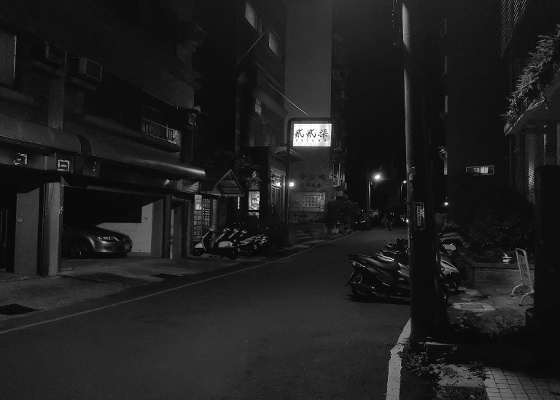
\includegraphics[width=0.7\textwidth]{src/sample3.png}
    \caption{\textbf{sample3.jpg}}
    \label{sample3}
\end{figure}


\subsection{(Bonus)}\label{2_bonus}
Try to replace the flowers in color or gray-scale \textbf{sample2.png} with \textbf{sample3.png} or other texture you prefer by using the result from (c), and output it as \textbf{result5.png}.

\paragraph{Approach}
My approach is
\begin{enumerate}
    \item Use the intermediates of cluster results, which means the \textbf{tags of each pixel}.
    \item Expand the \nameref{sample3} to \((450, 600)\) that larger than \nameref{sample2}.
    \item Replace the \textbf{tags of flowers} with \nameref{sample3}.
    \item Keep other tags as original \nameref{sample2}.
\end{enumerate}

\paragraph{Performance of results}

Result of problem 2(Bonus): \nameref{result5}
\begin{figure}
    \centering
    \includegraphics[width=0.7\textwidth]{src/result5.png}
    \caption{\textbf{result5.png} Texture replacement}
    \label{result5}
\end{figure}

\paragraph{Discussion}
Thanks to TA's advice. I try to expand the \nameref{sample3} that could be assigned to new figures.
But it still has some \textbf{strange boundaries} at \textbf{horizontal view}.
Maybe I could try better in future.

